\section{Persistenz}

\begin{concept}{Persistenz Grundlagen}\\
Persistenz bezeichnet die dauerhafte Speicherung von Daten über das Programmende hinaus:
\begin{itemize}
    \item Speicherung in Datenbankmanagementsystemen (DBMS)
    \item Haupttypen:
    \begin{itemize}
        \item Relationale Datenbanksysteme (RDBMS)
        \item NoSQL-Datenbanken (ohne fixes Schema)
    \end{itemize}
    \item O/R-Mapping (Object Relational Mapping)
    \begin{itemize}
        \item Abbildung zwischen Objekten und Datensätzen
        \item Überwindung des Strukturbruchs (Impedance Mismatch)
    \end{itemize}
\end{itemize}
\end{concept}

\begin{definition}{O/R-Mismatch}\\
Der Strukturbruch zwischen objektorientierter und relationaler Welt:
\begin{itemize}
    \item \textbf{Typen-Systeme:}
    \begin{itemize}
        \item Unterschiedliche NULL-Behandlung
        \item Datum/Zeit-Darstellung
    \end{itemize}
    \item \textbf{Beziehungen:}
    \begin{itemize}
        \item Richtung der Beziehungen
        \item Mehrfachbeziehungen
        \item Vererbung
    \end{itemize}
    \item \textbf{Identität:}
    \begin{itemize}
        \item OO: Implizite Objektidentität
        \item DB: Explizite Identität (Primary Key)
    \end{itemize}
\end{itemize}
\end{definition}

\subsection{JDBC - Java Database Connectivity}

\begin{concept}{JDBC Grundlagen}\\
JDBC ist die standardisierte Schnittstelle für Datenbankzugriffe in Java:
\begin{itemize}
    \item Seit JDK 1.1 (1997)
    \item Plattformunabhängig
    \item Datenbankunabhängig
    \item Aktuelle Version: 4.2
\end{itemize}
\end{concept}

\begin{KR}{JDBC Verwendung}
Grundlegende Schritte für Datenbankzugriff:
\begin{enumerate}
    \item JDBC-Treiber installieren und laden
    \item Verbindung zur Datenbank aufbauen
    \item SQL-Statements ausführen
    \item Ergebnisse verarbeiten
    \item Transaktion abschließen (Commit/Rollback)
    \item Verbindung schließen
\end{enumerate}
\end{KR}



\subsection{Design Patterns für Persistenz}

\begin{theorem}{Persistenz Design Patterns}\\
Drei grundlegende Ansätze für die Persistenzschicht:
\begin{itemize}
    \item \textbf{Active Record (Anti-Pattern):}
    \begin{itemize}
        \item Entität verwaltet eigene Persistenz
        \item Vermischung von Fachlichkeit und Technik
        \item Schlechte Testbarkeit
    \end{itemize}
    \item \textbf{Data Access Object (DAO):}
    \begin{itemize}
        \item Kapselung des Datenbankzugriffs
        \item Trennung von Fachlichkeit und Technik
        \item Gute Testbarkeit durch Mocking
    \end{itemize}
    \item \textbf{Repository (DDD):}
    \begin{itemize}
        \item Abstraktionsschicht über Data-Mapper
        \item Zentralisierung von Datenbankabfragen
        \item Komplexere Implementierung
    \end{itemize}
\end{itemize}
\end{theorem}

\begin{KR}{DAO Implementation}\\
Schritte zur Implementierung eines DAOs:
\begin{enumerate}
    \item Interface definieren:
    \begin{itemize}
        \item CRUD-Methoden (Create, Read, Update, Delete)
        \item Spezifische Suchmethoden
    \end{itemize}
    \item Domänenklasse erstellen:
    \begin{itemize}
        \item Nur fachliche Attribute
        \item Keine Persistenzlogik
    \end{itemize}
    \item DAO-Implementierung:
    \begin{itemize}
        \item Datenbankzugriff kapseln
        \item O/R-Mapping implementieren
        \item Transaktionshandling
    \end{itemize}
\end{enumerate}
\end{KR}



\subsection{Java Persistence API (JPA)}

\begin{concept}{JPA Grundkonzepte}\\
JPA ist der Java-Standard für O/R-Mapping:
\begin{itemize}
    \item \textbf{Entity-Klassen:}
    \begin{itemize}
        \item Plain Old Java Objects (POJOs)
        \item Annotation @Entity
        \item Keine JPA-spezifischen Abhängigkeiten
    \end{itemize}
    \item \textbf{Referenzen:}
    \begin{itemize}
        \item Eager/Lazy Loading
        \item Automatisches Nachladen
    \end{itemize}
    \item \textbf{Provider:}
    \begin{itemize}
        \item Hibernate
        \item EclipseLink
        \item OpenJPA
    \end{itemize}
\end{itemize}
\end{concept}

\begin{concept}{JPA Technologie-Stack}\\
\begin{itemize}
    \item Java Application
    \item Java Persistence API
    \item JPA Provider (Hibernate, EclipseLink, etc.)
    \item JDBC Driver
    \item Relationale Datenbank
\end{itemize}
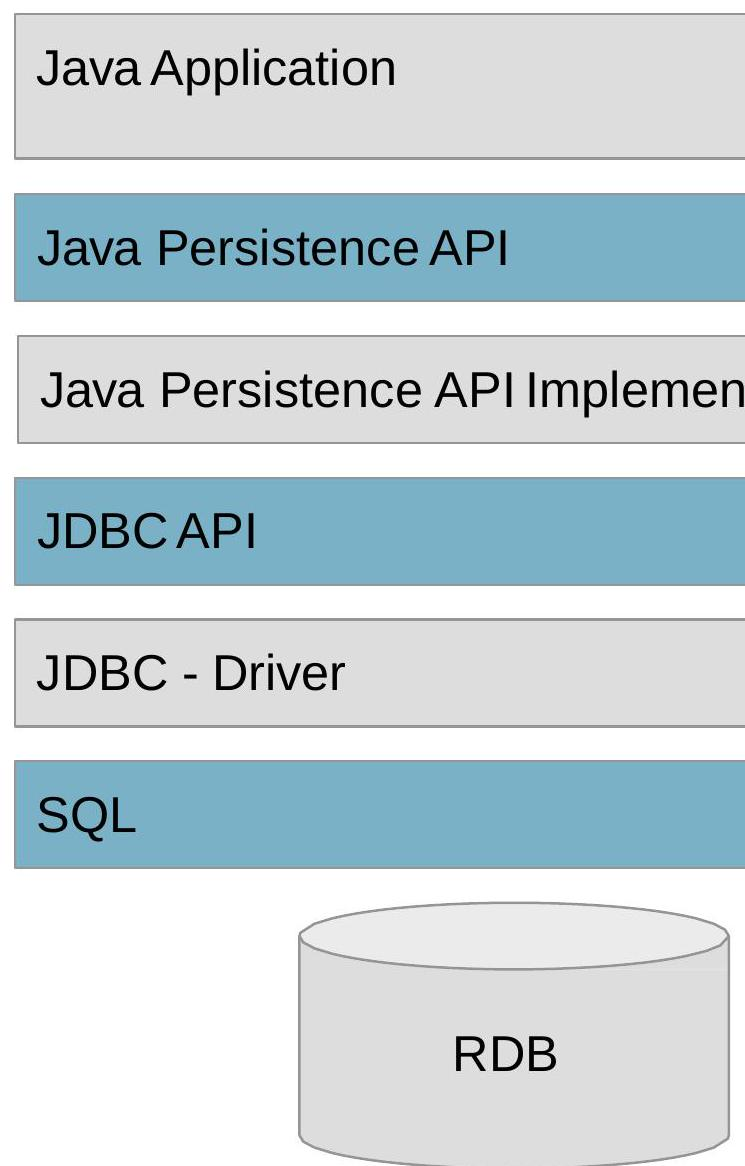
\includegraphics[width=0.8\linewidth]{images/2025_01_02_5ba1dc702e9f94ba8e06g-29.jpg}
\end{concept}

\begin{KR}{JPA Entity Erstellung}
\begin{enumerate}
    \item Entity-Klasse definieren:
    \begin{itemize}
        \item @Entity Annotation
        \item ID-Feld mit @Id markieren
    \end{itemize}
    \item Beziehungen definieren:
    \begin{itemize}
        \item @OneToMany, @ManyToOne etc.
        \item Navigationsrichtung festlegen
    \end{itemize}
    \item Validierung hinzufügen:
    \begin{itemize}
        \item @NotNull, @Size etc.
        \item Geschäftsregeln
    \end{itemize}
\end{enumerate}
\end{KR}



\subsection{Repository Pattern}

\begin{concept}{Repository Pattern}\\
Das Repository Pattern bietet eine zusätzliche Abstraktionsschicht über der Data-Mapper-Schicht:
\begin{itemize}
    \item Zentralisierung von Datenbankabfragen
    \item Domänenorientierte Schnittstelle
    \item Unterstützung komplexer Abfragen
    \item Häufig in Kombination mit Spring Data
\end{itemize}
\end{concept}



\begin{remark}
Spring Data unterstützt die automatische Generierung von Repository-Implementierungen basierend auf Methodennamen. Dies reduziert den Implementierungsaufwand erheblich.
\end{remark}

\begin{example}{Prüfungsaufgabe: O/R-Mapping Analyse}
\textbf{Szenario:}
Ein Universitätssystem verwaltet Studenten, Kurse und Noten. Studenten können mehrere 
Kurse belegen, ein Kurs hat mehrere Studenten.

\textbf{Aufgabe:} 
Analysieren Sie die O/R-Mapping Herausforderungen dieser Domain.

\textbf{Lösung:}
\begin{itemize}
    \item \textbf{Beziehungen:}
    \begin{itemize}
        \item Many-to-Many zwischen Student und Kurs
        \item Zusätzliche Attribute in der Beziehung (Noten)
        \item Bidirektionale Navigation erforderlich
    \end{itemize}
    
    \item \textbf{Vererbung:}
    \begin{itemize}
        \item Person -> Student/Dozent
        \item Verschiedene Mapping-Strategien möglich
    \end{itemize}
    
    \item \textbf{Komplexe Daten:}
    \begin{itemize}
        \item Adressdaten als Wertobjekte
        \item Zeiträume für Kursbelegung
    \end{itemize}
\end{itemize}
\end{example}

\begin{KR}{Persistenzstrategie wählen}
\textbf{1. Anforderungen analysieren}
\begin{itemize}
    \item \textbf{Funktional:}
    \begin{itemize}
        \item Datenmodell-Komplexität
        \item Abfrageanforderungen
        \item Transaktionsverhalten
    \end{itemize}
    \item \textbf{Nicht-funktional:}
    \begin{itemize}
        \item Performance
        \item Skalierbarkeit
        \item Wartbarkeit
    \end{itemize}
\end{itemize}

\textbf{2. Technologien evaluieren}
\begin{itemize}
    \item \textbf{JDBC:}
    \begin{itemize}
        \item Direkte Kontrolle
        \item Hohe Performance
        \item Hoher Implementierungsaufwand
    \end{itemize}
    \item \textbf{JPA:}
    \begin{itemize}
        \item Standardisiert
        \item Produktiv
        \item Lernkurve
    \end{itemize}
    \item \textbf{NoSQL:}
    \begin{itemize}
        \item Flexibles Schema
        \item Hohe Skalierbarkeit
        \item Spezielle Anwendungsfälle
    \end{itemize}
\end{itemize}
\end{KR}

\begin{example}{Prüfungsaufgabe: Design Pattern Vergleich}
\textbf{Aufgabe:}
Vergleichen Sie Active Record, DAO und Repository Pattern.

\textbf{Analysematrix:}
\begin{itemize}
    \item \textbf{Active Record:}
    \begin{itemize}
        \item \textbf{Vorteile:}
        \begin{itemize}
            \item Einfache Implementierung
            \item Schnell zu entwickeln
        \end{itemize}
        \item \textbf{Nachteile:}
        \begin{itemize}
            \item Keine Trennung der Belange
            \item Schlechte Testbarkeit
            \item Vermischung von Fachlogik und Persistenz
        \end{itemize}
    \end{itemize}
    
    \item \textbf{DAO:}
    \begin{itemize}
        \item \textbf{Vorteile:}
        \begin{itemize}
            \item Klare Trennung der Belange
            \item Gute Testbarkeit
            \item Austauschbare Implementierung
        \end{itemize}
        \item \textbf{Nachteile:}
        \begin{itemize}
            \item Mehr Initialaufwand
            \item Zusätzliche Abstraktionsebene
        \end{itemize}
    \end{itemize}
    
    \item \textbf{Repository:}
    \begin{itemize}
        \item \textbf{Vorteile:}
        \begin{itemize}
            \item Domänenorientierte Schnittstelle
            \item Zentrale Abfragelogik
            \item DDD-konform
        \end{itemize}
        \item \textbf{Nachteile:}
        \begin{itemize}
            \item Komplexere Implementierung
            \item Höhere Lernkurve
        \end{itemize}
    \end{itemize}
\end{itemize}
\end{example}

\begin{KR}{JPA Entity Design}
\textbf{1. Grundstruktur}
\begin{itemize}
    \item \textbf{Basisanforderungen:}
    \begin{itemize}
        \item Default Constructor
        \item Serializable (optional)
        \item Getter/Setter
    \end{itemize}
    \item \textbf{Identifikation:}
    \begin{itemize}
        \item Primary Key Strategie
        \item Natural vs. Surrogate Key
    \end{itemize}
\end{itemize}

\textbf{2. Beziehungen}
\begin{itemize}
    \item \textbf{Kardinalität:}
    \begin{itemize}
        \item OneToOne
        \item OneToMany/ManyToOne
        \item ManyToMany
    \end{itemize}
    \item \textbf{Richtung:}
    \begin{itemize}
        \item Unidirektional
        \item Bidirektional
    \end{itemize}
    \item \textbf{Lifecycle:}
    \begin{itemize}
        \item Cascade-Operationen
        \item Orphan Removal
    \end{itemize}
\end{itemize}

\textbf{3. Optimierungen}
\begin{itemize}
    \item \textbf{Lazy Loading:}
    \begin{itemize}
        \item Fetch-Strategien
        \item Join Fetching
    \end{itemize}
    \item \textbf{Caching:}
    \begin{itemize}
        \item First-Level Cache
        \item Second-Level Cache
    \end{itemize}
\end{itemize}
\end{KR}

[Previous content about Repository Pattern remains]